\chapter{Node.js}

\section{Wprowadzenie}
W poniższym rozdziale przedstawione zostaną podstawowe aspekty użycia frameworka \textit{Node.js} z wykorzystaniem zestawu bibliotek oferowanych przez \textit{Express.js} oraz sposób implementacji i analiza działania prostej aplikacji serwerowej, której zadaniem będzie prezentacja uzyskanych wyników. Aplikacja serwerowa pracuje na środowisku lokalnym, na porcie 9000. Wiąże się to z koniecznością przekierowywania wszelkich aplikacji klienckich na ten właśnie port. Dane przechowywane są w plikach dołączonych do projektu. Ogólny schemat aplikacji klient-serwer przedstawiony został na rysunku \ref{Rys:nodejs}.

\begin{figure}[h]
	\centering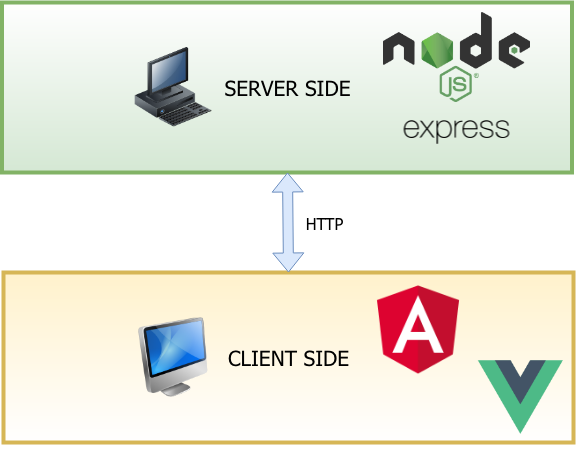
\includegraphics[scale=0.5]{images/nodejs.png}
	\caption{Ogólny schemat działania aplikacji typu klient-serwer bazującej na serwerze \textit{Node.js} oraz nowoczesnych frameworkach implementacji warstwy prezentacji}
	\label{Rys:nodejs}
\end{figure}

\section{Implementacja aplikacji serwerowej}
W poniższym rozdziale przedstawiony zostanie sposób implementacji aplikacji serwerowej bazującej na zestawie bibliotek \textit{Node.js} oraz \textit{Express.js}.

\subsection{Inicjalizacja serwera}
Inicjalizacja serwera rozpoczyna się od wygenerowania klucza i certyfikatu SSL (\textit{Secure Socket Layer}), który używany jest przez protokół HTTPS w celu zwiększenia bezpieczeństwa danych. Kolejnym krokiem jest zdefiniowanie portu, na którym będzie on nasłuchiwał żądań klienta i rozpoczęcia nasłuchiwania. W tym celu posłużono się frameworkiem \textit{Express.js} i zdefiniowano lokalny serwer HTTPS pracujący na porcie numer 9000. 

W celu wygenerowania certyfikatu i klucza RSA (\textit{Rivest-Shamir-Adleman}) posłużono się poniższą komendą:

\begin{verbatim}
openssl req -newkey rsa:2048 -new -nodes -keyout key.pem -out cert.pem
\end{verbatim}

Wygenerowany klucz RSA zawiera 2048 bitów. Rozmiar ten wybrany został z kilku powodów. Przede wszystkim wiele urządzeń nie wspiera większych wartości bitowych. Ponadto, użycie tego klucza w trakcie szyfrowania i uwierzytelniania powoduje znacznie mniejsze zużycie procesora. 

Sama, wstępna implementacja serwera HTTPS i przekazanie wygenerowanych plików \textit{key.pem} oraz \textit{cert.pem} do parametrów inicjalizacji serwera  zaprezentowana została na poniższych blokach kodu źródłowego:

\begin{verbatim}
const httpsServer = https.createServer({
key: fs.readFileSync('key.pem'),
cert: fs.readFileSync('cert.pem')
}, app);

httpServer = app.listen(9000, () => {
console.log("HTTP Server running at https://localhost:" + 
httpServer.address().port);
});
\end{verbatim}

W następnym kroku zdefiniowano komendę \textit{start-server}, za pomocą której uruchamiany będzie serwer. Definicja komendy znajduje się w pliku JSON służącym do zarządzania lokalnymi paczkami NPM (\textit{Node Package Module}) - \textit{package.json}. W celu uruchomienia serwera wystarczy użyć polecenia \textit{npm run start-server}. 

\begin{verbatim}
	"start-server": "./node_modules/.bin/ts-node ./server/server.ts --secure",
\end{verbatim}

Po uruchomieniu serwera z poziomu konsoli otrzymano komunikat widoczny na rysunku \ref{Rys:nodejs-running}.

\begin{figure}[h]
	\centering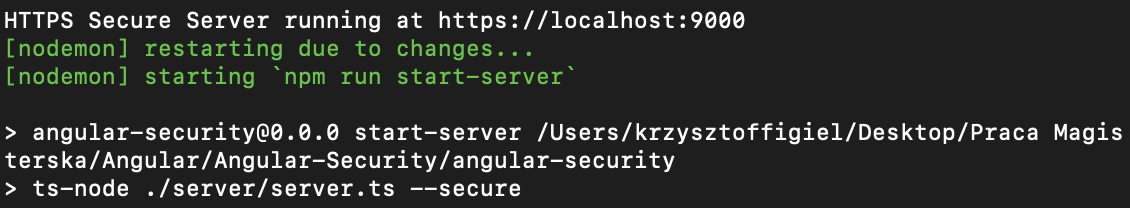
\includegraphics[scale=0.76]{images/nodejs/server-running.png}
	\caption{Zrzut ekranu konsoli systemu \textit{MacOS} ukazujący komunikaty o poprawnym uruchomieniu procesu nasłuchiwania przez serwer na porcie 9000}
	\label{Rys:nodejs-running}
\end{figure}

Definicja tabel routingu w \textit{Express.js} opiera się na użyciu funkcji \texttt{app.route(path)}. W aplikacji serwerowej zdefiniowano następujące ścieżki routingu:

\begin{itemize}
	\item \textit{/api/books}
	\item \textit{/api/signup}
	\item \textit{/api/user}
	\item \textit{/api/logout}
	\item \textit{/api/login}
\end{itemize}

Przykładowa definicja wpisu tabeli routingu zaprezentowana została na poniższym bloku kodu źródłowego:

\begin{verbatim}
app.route('/api/books')
.get(readAllBooks);
\end{verbatim}

\subsection{Implementacja modułu rejestracji nowego użytkownika} 
W następnym kroku zdefiniowano metody odpowiedzialne za obsługę rejestracji nowego użytkownika w aplikacji. Wpis tabeli routingu zawierający ścieżkę do tworzenia nowego użytkownika wygląda następująco:

\begin{verbatim}
app.route('/api/signup')
.post(createUser);
\end{verbatim}

Po zdefiniowaniu wpisu przystąpiono do implementacji metody \texttt{createUser(req, res)}. Sama implementacja tej metody opiera się na odebraniu parametrów przesyłanych przez użytkownika w obiekcie \texttt{req} i przekazania odpowiednich statusów metody HTTP do klienta (\texttt{res}) w zależności czy weryfikacja nowego użytkownika przebiegła pomyślnie czy też nie. 

Do walidacji haseł użytkownika posłużono się walidatorem z repozytorium NPM - \textit{password-validator}. Umożliwia on zdefiniowanie reguł tworzenia nowych haseł oraz dodawanie haseł, które znaleźć się mają na tzw. \textit{blacklist} czyli liście haseł niedopuszczalnych, powszechnie używanych. W celu zachowania bezpieczeństwa systemu zdefiniowano reguły i przykład \textit{blacklist} tworzenia nowych haseł przez użytkowników:

\begin{verbatim}
schema
.is().min(10)                                   // Minimum length 10
.has().uppercase()                              // Must have uppercase letters
.has().lowercase()                              // Must have lowercase letters
.has().digits()                                 // Must have digits
.has().not().spaces()                           // Should not have spaces
.is().not().oneOf(['Passw0rd', 'Password123']); // Blacklist these values
\end{verbatim}

Po pomyślnej walidacji przesyłanego przez użytkownika w obiekcie \texttt{req} hasła serwer odpowiada komunikatem 200 przesyłając w parametrze \texttt{body} dane (\textit{id} oraz \textit{email}) nowego użytkownika. W tym celu posłużono się metodą \texttt{res.status(httpCode)}:

\begin{verbatim}
res.status(200).json({ id: user.id, email: user.email });
\end{verbatim}

W przypadku podania hasła nieazgodnego z przyjętymi regułami tworzenia nowych haseł użytkownika serwer odpowiada komunikatem 400 \textit{Bad request}. Wykorzystano metodę \texttt{res.status(httpCode)}, a jako zwracany parametr podano listę błędów zwracaną przez pakiet \textit{password-validator}:

\begin{verbatim}
res.status(400).json({ errors });
\end{verbatim}

Jeżeli serwer napotkał wewnętrzny błąd, wówczas wysyła on komunikat o kodzie 500 \textit{Internal Server Error} za pomocą metody \texttt{res.sendStatus(httpCode)} bez przekazywania treści błędu w celu zachowania odpowiedniej hermetyzacji aplikacji:

\begin{verbatim}
res.sendStatus(500);
\end{verbatim}

Nowi użytkownicy przechowywani są w bazie danych za pomocą obiektu składającego się z trzech wartości:

\begin{verbatim}
const user: DbUser = {
id,
email,
passwordDigest
};
\end{verbatim}

Przy tworzeniu nowego użytkownika sprawdzany jest dodatkowo warunek czy nie ma już podobnego konta w bazie danych:

\begin{verbatim}
const usersPerEmail = _.keyBy(_.values(USERS), 'email');

if (usersPerEmail[email]) {
const message = 'User already exists with assigned email address: ' + email;
console.error(message);
throw new Error(message);
}
\end{verbatim}

Jeżeli użytkownik istnieje w bazie danych wyświetlany jest stosowny komunikat. W przypadku braku podobnego konta i pomyślnej weryfikacji tworzony i zwracany jest nowy obiekt \texttt{user}:

\begin{verbatim}
this.userCounter++;

const id = this.userCounter++;

const user: DbUser = {
id,
email,
passwordDigest
};

USERS[id] = user;

return user;
\end{verbatim}

Hasła użytkownika przechowywane są w bazie danych za pomocą funkcji skrótu \textit{Argon2}. W tym celu wykorzystano specjalny pakiet oferowany przez repozytorium NPM. Hasło podane przez użytkownika przekazywane jest jako parametr funkcji \texttt{argon2.hash(\textit{password})}. Więcej informacji na temat wykorzystania funkcji \textit{Argon2} zawarte zostało w rozdziale dotyczącym bezpieczeństwa. 

\subsection{Implementacja modułu logowania użytkownika}

\subsection{Implementacja modułu wylogowywania użytkownika}

\subsection{Implementacja mechanizmów podtrzymywania sesji użytkownika}
